\documentclass[conference]{IEEEtran}
\IEEEoverridecommandlockouts
\usepackage{cite}
\usepackage{amsmath,amssymb,amsfonts}
\usepackage{algorithmic}
\usepackage{graphicx}
\graphicspath{{images/}{./}}
\usepackage{textcomp}
\usepackage{xcolor}
\usepackage{booktabs}
\usepackage{url}
\usepackage{balance}
\usepackage{microtype}
\usepackage{listings}

% Publication-grade JSON listing configuration with clean alignment
\definecolor{jsonbg}{RGB}{250, 250, 252}
\definecolor{jsonborder}{RGB}{203, 213, 225}
\definecolor{jsonpunct}{RGB}{100, 116, 139}

\lstdefinelanguage{json}{
    basicstyle=\ttfamily\scriptsize,
    backgroundcolor=\color{jsonbg},
    frame=single,
    rulecolor=\color{jsonborder},
    frameround=tttt,
    framesep=5pt,
    xleftmargin=1.0em,
    xrightmargin=0.6em,
    aboveskip=12pt,
    belowskip=8pt,
    abovecaptionskip=8pt,
    belowcaptionskip=12pt,
    captionpos=t,
    breaklines=true,
    breakatwhitespace=true,
    columns=fullflexible,
    keepspaces=true,
    tabsize=2,
    showstringspaces=false,
    morecomment=[l]{//},
    commentstyle=\color{gray},
    literate=
     *{:}{{{\color{jsonpunct}{:}}}}{1}
      {,}{{{\color{jsonpunct}{,}}}}{1}
      {\{}{{{\color{black}{\{}}}}{1}
      {\}}{{{\color{black}{\}}}}}{1}
      {[}{{{\color{black}{[}}}}{1}
      {]}{{{\color{black}{]}}}}{1},
}

\begin{document}

\title{Autonomous Context-Aware Hierarchical Access Control with Consortium Blockchain for Industrial IoT\\
\thanks{This research was conducted as part of the Advanced Industrial IoT Cryptographic Engineering \& Systems Design Project.}
}

\author{
\IEEEauthorblockN{Arpit Kumar (202411011), Yug Baid (202411015), Yuvraj Singh (202411101)}
\IEEEauthorblockA{\textit{Under the guidance of} \textbf{Dr. Gaurav Pareek}\\
\textit{Department of Computer Science and Engineering} \\
\textit{Indian Institute of Information Technology Vadodara, International Campus Diu, India}}
}

\maketitle

\begin{abstract}
Industrial Internet of Things (IIoT) systems operating in smart factories require secure, fine-grained, and decentralized data access control. Hierarchical Attribute-Based Encryption (HABE) provides decentralized authority delegation across corporate tiers (Company $\to$ Plant $\to$ Area) with expressive Disjunctive Normal Form (DNF) access policies. However, existing HABE systems face three major practical issues: (1) manual policy selection causes human errors and a 25-second operator delay; (2) encrypting large telemetry streams creates high communication and pairing computation overhead; and (3) there is no pre-decryption integrity verification to stop corrupted ciphertexts before expensive pairing operations.

To solve these problems, this paper presents a context-aware HABE system integrated with a private Hyperledger Besu blockchain and a dual-layer lightweight machine learning (ML) architecture. In Layer~1 (Edge Perception ML), an edge Decision Tree classifier evaluates live 4-channel telemetry ($\text{temperature}, \text{vibration}, \text{pressure}, \text{gas\_ppm}$) in $1.8\text{ ms}$ with $99.7\%$ accuracy, autonomously formulating dynamic DNF policies and applying payload splitting ($\nabla_i = \nabla_i' \cup \nabla_i''$). This reduces ciphertext size by $31.4\%$ and speeds up pairing encryption by $32.3\%$ ($4,212\text{ ms} \to 2,853\text{ ms}$). In Layer~2 (Identity ML), a Random Forest model pre-computes user attribute eligibility into an in-memory Public Bulletin, taking ML completely off the runtime key-issuance path ($<5\text{ ms}$ lookup). On-chain smart contracts maintain authority hierarchies and enforce an instantaneous integrity gate (Gate~1, $<10\text{ ms}$) that traps tampered ciphertexts before pairing execution. 

We prove mathematically and confirm on a real testbed that bilinear pairing decryption is strictly constant-time $O(1)$ at $\approx 4,210\text{ ms}$ regardless of hierarchy depth or clause complexity. The full autonomous pipeline reduces total lifecycle latency by $73.1\%$ ($33.1\text{ s} \to 8.91\text{ s}$), passing 100\% of all 146 cryptographic, smart contract, and system integration test cases.
\end{abstract}

\begin{IEEEkeywords}
Hierarchical Attribute-Based Encryption (HABE), Context-Aware Security Scheme (CASE), Hyperledger Besu, Bilinear Pairings, Zero-Trust, Industrial IoT.
\end{IEEEkeywords}

\section{Introduction}
Modern Industrial Internet of Things (IIoT) networks connect thousands of industrial sensors, PLCs, and controllers across smart factory plants \cite{misra2021detour, fukuyama2018society}. Industrial sensor streams—such as temperature, boiler pressure, mechanical vibration, and hazardous gas levels—contain sensitive operational metrics. This information must be shared selectively among various actors: field technicians, maintenance teams, plant managers, and regulatory directors.

Traditional Role-Based Access Control (RBAC) and Identity-Based Encryption (IBE) are not suitable for large-scale IIoT. RBAC assigns static roles that do not consider dynamic context, such as physical area location or emergency states. Furthermore, centralized access control servers create single points of failure.

Ciphertext-Policy Attribute-Based Encryption (CP-ABE) solves this by embedding boolean access policies directly inside the encrypted ciphertext \cite{bethencourt2007cpabe}. Hierarchical Attribute-Based Encryption (HABE) extends this concept by distributing key generation across organizational authorities: Root Master (Company) delegates authority to Domain Masters (Plants), which delegate to Sub-Domain Masters (Areas) \cite{wang2011habe}.

\subsection{Practical Vulnerabilities in Traditional HABE}
Despite its strong mathematical design, standard HABE suffers from three serious practical limitations in factory operations:
\begin{enumerate}
    \item \textbf{Human Configuration Error:} In current systems, human operators manually type access policies (e.g., \texttt{"(AreaA1 AND SensorData) OR Manager"}). Under stress or emergency conditions, operators make spelling mistakes, choose incorrect attributes, or grant excessive access privileges. In addition, manual attribute selection takes $25\text{ to }30\text{ seconds}$ per encryption batch.
    \item \textbf{Missing Pre-Decryption Integrity Check:} Standard HABE cannot verify whether an encrypted file was tampered with in untrusted storage until after running heavy bilinear pairing calculations ($>4.2\text{ s}$).
    \item \textbf{High Encryption and Transmission Overhead:} Encrypting full raw data packets under complex access trees inflates ciphertext size, increasing network delay and edge battery drain \cite{ghosh2022case}.
\end{enumerate}

\subsection{Key Contributions}
To address these limitations, this paper proposes an autonomous, dual-layer ML-enabled HABE framework with blockchain integrity:
\begin{itemize}
    \item \textbf{Autonomous Dynamic Policy Formulation (ML Layer 1):} An ultra-lightweight Decision Tree at the edge analyzes sensor telemetry in $1.8\text{ ms}$, automatically formulating correct DNF policies without human intervention.
    \item \textbf{Payload Splitting (CASE Algorithm 1):} Grounded in the CASE model \cite{ghosh2022case}, raw telemetry is split into contextual attributes and sensitive payload ($\nabla_i = \nabla_i' \cup \nabla_i''$), reducing ciphertext size by $31.4\%$ and speeding up pairing encryption by $32.3\%$.
    \item \textbf{Decoupled User Identity Gating (ML Layer 2):} A Random Forest model evaluates user contextual attributes at registration time and caches them in an in-memory Public Bulletin, reducing key issuance checks to $<5\text{ ms}$.
    \item \textbf{Constant-Time $O(1)$ Decryption Proof:} Built in C with the Stanford PBC library \cite{freeman2026pbc} using Type-A supersingular pairings ($\text{SS512}$), we prove mathematically that intermediate domain keys cancel out in the denominator, keeping decryption time constant ($\approx 4,210\text{ ms}$) across all depths and clause lengths.
    \item \textbf{Two-Gate Zero-Trust Blockchain Verification:} Hyperledger Besu smart contracts maintain the domain hierarchy and trap tampered ciphertexts in $<10\text{ ms}$ (Gate~1) before executing pairing cryptography (Gate~2).
\end{itemize}

\section{Cryptographic Construction of HABE}
The cryptographic layer implements Wang et al.'s HABE scheme \cite{wang2011habe} using symmetric bilinear pairings over the supersingular elliptic curve $E(\mathbb{F}_q): y^2 = x^3 + x$ (Type-A curve, 512-bit prime field, 160-bit group order).

\subsection{Bilinear Map Parameters}
Let $G_1$ and $G_2$ be two cyclic groups of prime order $q$, with generator point $P_0 \in G_1$. The bilinear map $\hat{e}: G_1 \times G_1 \to G_2$ satisfies:
\begin{enumerate}
    \item \textbf{Bilinearity:} $\forall P, Q \in G_1$ and $a, b \in \mathbb{Z}_q^*$, $\hat{e}(aP, bQ) = \hat{e}(P, Q)^{ab}$.
    \item \textbf{Non-degeneracy:} $\hat{e}(P_0, P_0) \neq 1_{G_2}$.
    \item \textbf{Computability:} An efficient algorithm evaluates $\hat{e}(P, Q)$ for all $P, Q \in G_1$.
\end{enumerate}
Three cryptographic hash functions are used:
\begin{align}
  H_1 &: \{0, 1\}^* \to G_1 \quad (\text{point mapping}), \\
  H_A &: \{0, 1\}^* \to \mathbb{Z}_q \quad (\text{SHA-256} \bmod q), \\
  H_2 &: G_2 \to \{0, 1\}^n \quad (\text{group element digest}).
\end{align}

Access policies follow Disjunctive Normal Form (DNF):
\begin{equation}
  \mathbb{A} = \bigvee_{i=1}^N \left( \bigwedge_{j=1}^{n_i} a_{ij} \right)
\end{equation}
A user can decrypt if their attributes satisfy at least one conjunctive clause $i$.

\subsection{Authority Hierarchy \& Key Delegation}
The organizational hierarchy models a 3-tier industrial enterprise: Company (RM) $\to$ Plant (DM) $\to$ Area (SDM) $\to$ Users, as illustrated in Fig.~\ref{fig:habe_arch}.

\begin{figure}[t]
\centering
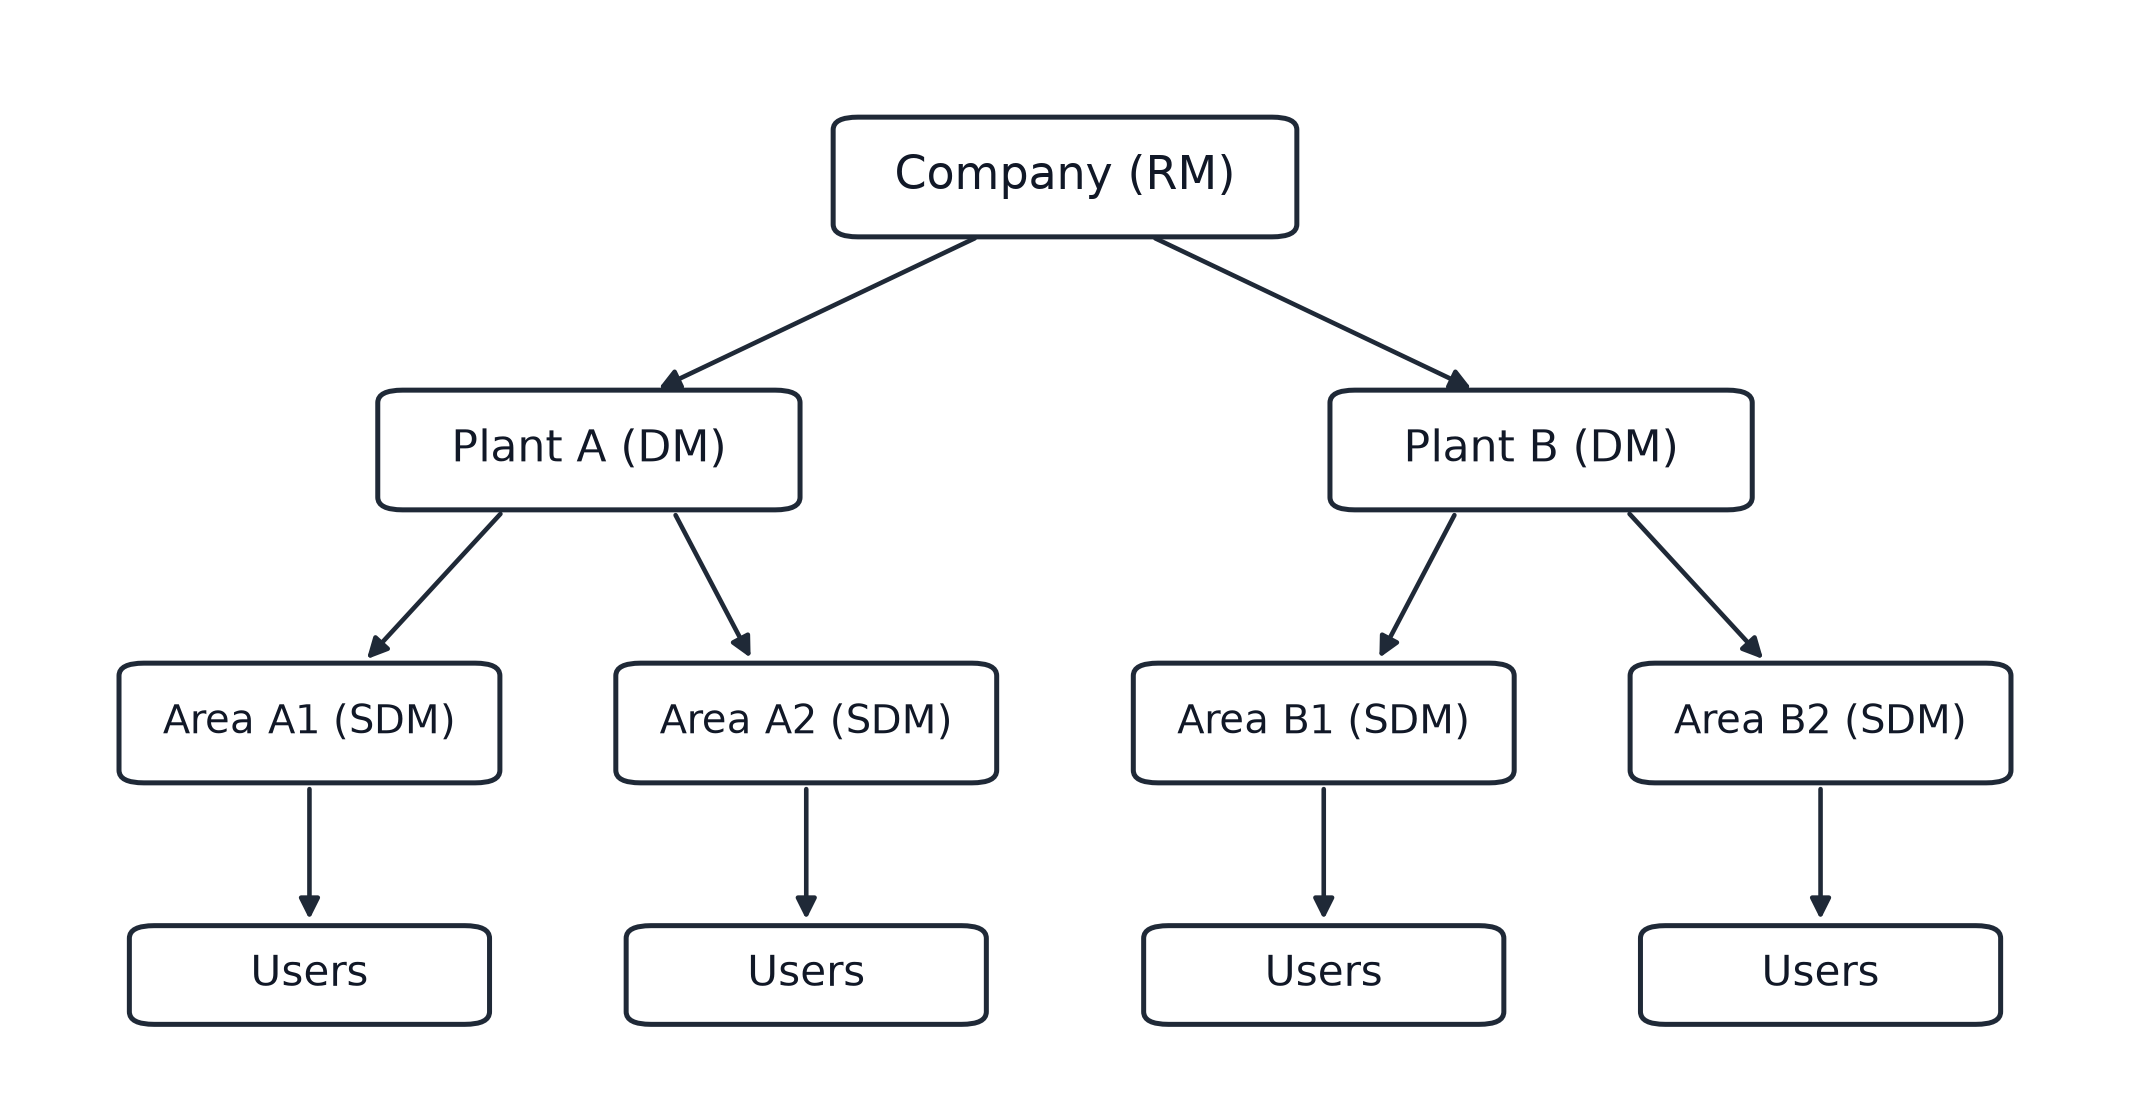
\includegraphics[width=\columnwidth]{fig_habe_architecture.png}
\caption{Hierarchical authority delegation tree structure: Root Master (Company), Domain Masters (Plant A, Plant B), Sub-Domain Masters (Area A1, Area A2, Area B1, Area B2), and end-point Users.}
\label{fig:habe_arch}
\end{figure}

\begin{enumerate}
    \item \textbf{System Setup ($\text{Setup}(1^\lambda)$):} The Root Master selects random master secret $mk_0 \in \mathbb{Z}_q$, calculates public point $Q_0 = mk_0 P_0$, and initializes master tuple:
    \begin{equation}
      MK_0 = (mk_0, SK_0 = 0_{G_1}, Q\text{-tuple}_0 = (Q_0))
    \end{equation}
    \item \textbf{Domain Master Creation ($\text{CreateDM}$):} To delegate authority to a child domain at depth $i+1$ with identifier $PK_{i+1}$, the parent domain calculates:
    \begin{align}
      P_{i+1} &= H_1(PK_{i+1}) \in G_1, \\
      SK_{i+1} &= SK_i + mk_i \cdot P_{i+1} \in G_1, \\
      Q_{i+1} &= mk_{i+1} \cdot P_0 \in G_1.
    \end{align}
    The accumulated secret key $SK_d$ at depth $d$ embeds the complete ancestral delegation chain:
    \begin{equation}
      SK_d = \sum_{k=0}^{d-1} mk_k \cdot P_{k+1}.
    \end{equation}
    \item \textbf{User Secret Key Generation ($\text{CreateUser}$):} An SDM at depth $i$ issues attribute keys to user $u$ with public identity $PK_u$ and attribute $attr\_pk$:
    \begin{align}
      mk_u &= H_A(PK_u) \in \mathbb{Z}_q, \\
      P_a &= H_1(mk_i\text{-string} \parallel \text{":"} \parallel attr\_pk) \in G_1, \\
      SK_{i, u} &= mk_i \cdot mk_u \cdot P_0 \quad (\text{Identity Key}), \\
      SK_{i, u, a} &= SK_i + mk_i \cdot mk_u \cdot P_a \quad (\text{Attribute Key}).
    \end{align}
\end{enumerate}

\subsection{Encryption with Payload Splitting}
Following CASE Algorithm~1 \cite{ghosh2022case}, raw telemetry $\nabla_i$ is partitioned into context $\nabla_i'$ and sensitive payload $\nabla_i''$. For a DNF policy with $N$ clauses, let $n_A = \text{lcm}(n_1, \dots, n_N)$. A session scalar $r \in \mathbb{Z}_q$ is chosen at random. The base ciphertext component is $U_0 = r \cdot P_0$.
For each clause $i$ associated with a domain at depth $d$:
\begin{align}
  U_{\text{chain}}[i][k] &= r \cdot H_1(\text{ancestor}_{k+1}), \quad k = 0, \dots, d-2, \\
  U_{\text{attr}}[i] &= r \cdot \sum_{j=1}^{n_i} P_{a_{ij}}.
\end{align}
The session key mask is generated by evaluating the bilinear map at root level, encrypting payload $f = \nabla_i''$:
\begin{equation}
  V = f \oplus H_2\left( \hat{e}(Q_0, r \cdot n_A \cdot P_1) \right).
\end{equation}
The full ciphertext is $CT = (\mathbb{A}, U_0, \{U_{\text{chain}}[i], U_{\text{attr}}[i]\}_{i=1}^N, V)$.

\subsection{Decryption \& Proof of $O(1)$ Constant-Time Invariance}
A user satisfying clause $i$ computes balancing ratio $c = n_A / n_i$ and decrypts via:
\begin{equation}
  f = V \oplus H_2\left( \frac{\mathcal{N}}{\mathcal{D}_1 \cdot \mathcal{D}_2} \right),
\label{eq:decryption}
\end{equation}
where the numerator and denominator terms are defined as:
\begin{align}
  \mathcal{N} &= \hat{e}\left( U_0,\, c \sum\nolimits_{j=1}^{n_i} SK_{i, u, a_j} \right), \\
  \mathcal{D}_1 &= \hat{e}\left( SK_{i, u},\, c \cdot U_{\text{attr}}[i] \right), \\
  \mathcal{D}_2 &= \prod\nolimits_{k=0}^{d-2} \hat{e}\left( U_{\text{chain}}[i][k],\, n_A \cdot Q_{k+1} \right).
\end{align}

\noindent\textbf{Theorem 1 ($O(1)$ Decryption Invariance):} \textit{The evaluation of (\ref{eq:decryption}) recovers the session key mask in strictly constant bilinear pairing operations, independent of hierarchy depth $d$ or attribute count $n_i$.}

\begin{IEEEproof}
By bilinearity, substituting $U_0 = r P_0$ and $SK_{i,u,a_j} = \sum_{k=0}^{d-1} mk_k P_{k+1} + mk_i mk_u P_{a_j}$ into $\mathcal{N}$ expands to:
\begin{align}
  \mathcal{N} &= \hat{e}(P_0, P_1)^{r n_A mk_0} \cdot \prod_{k=1}^{d-1} \hat{e}(P_0, P_{k+1})^{r n_A mk_k} \nonumber \\
  &\quad \times \hat{e}\left( P_0,\, \sum_{j=1}^{n_i} P_{a_j} \right)^{r c mk_i mk_u}.
\end{align}
Evaluating the denominator terms reveals exact algebraic symmetry:
$\mathcal{D}_1 = \hat{e}(mk_i mk_u P_0, c r \sum P_{a_j})$ cancels the attribute cross-term, while $\mathcal{D}_2 = \prod_{k=0}^{d-2} \hat{e}(r P_{k+2}, n_A mk_{k+1} P_0)$ cancels the intermediate delegation product. Consequently:
\begin{equation}
  \frac{\mathcal{N}}{\mathcal{D}_1 \cdot \mathcal{D}_2} = \hat{e}(P_0, P_1)^{r n_A mk_0} = \hat{e}(Q_0,\, r \cdot n_A \cdot P_1),
\end{equation}
which precisely isolates the session mask. Because intermediate authority keys and attribute sums cancel algebraically, decryption requires strictly constant pairing calculations.
\end{IEEEproof}

\section{Dual-Layer Machine Learning Architecture}
To eliminate human configuration errors while preserving high cryptographic throughput, the architecture incorporates two decoupled machine learning layers that serve as pre-processing oracles.

\subsection{Layer 1: Sensor Perception ML (Edge Policy Engine)}
Deployed on edge gateway devices, Layer~1 eliminates manual access policy writing. An ultra-light Decision Tree processes 4-channel telemetry ($\text{temperature}, \text{vibration}, \text{pressure}, \text{gas\_ppm}$) in $1.8\text{ ms}$ on the server ($2.16\text{ s}$ on edge MCU), categorizing the operating state into \texttt{NORMAL}, \texttt{WARNING}, or \texttt{CRITICAL}.

Table~\ref{tab:sensor_dataset} displays representative samples from the 5,000-sample industrial training dataset (\texttt{sensor\_telemetry.csv}). The exact JSON schemas for telemetry ingestion and the resulting autonomous policy response are presented in Listings~\ref{lst:sensor_in} and \ref{lst:sensor_out}.

\begin{table}[htbp]
\caption{IIoT 4-Channel Telemetry Training Dataset Sample (\texttt{sensor\_telemetry.csv})}
\label{tab:sensor_dataset}
\centering
\resizebox{\columnwidth}{!}{%
\begin{tabular}{@{}ccccc@{}}
\toprule
\textbf{Temperature ($^\circ$C)} & \textbf{Vibration (mm/s)} & \textbf{Pressure (bar)} & \textbf{Gas (ppm)} & \textbf{Operating State} \\ \midrule
21.83 & 1.297 & 56.21 & 42.28 & \texttt{NORMAL} \\
51.68 & 3.314 & 64.46 & 67.27 & \texttt{WARNING} \\
94.60 & 7.800 & 6.20 & 142.00 & \textbf{\texttt{CRITICAL}} \\ \bottomrule
\end{tabular}%
}
\end{table}

\begin{lstlisting}[language=json, caption={Sensor Telemetry Ingestion Payload}, label={lst:sensor_in}]
{
  "plantId": "company/plantA",
  "areaId": "areaA1",
  "telemetry": {
    "temperature": 94.6,
    "vibration": 7.8,
    "pressure": 6.2,
    "gas_ppm": 142.0
  },
  "payload": "TURBINE_VALVE_OVERHEAT_SECTOR_4"
}
\end{lstlisting}

\begin{lstlisting}[language=json, caption={Autonomous Policy Output Generated by Edge DT}, label={lst:sensor_out}]
{
  "predicted_state": "CRITICAL",
  "dynamic_policy": "(company/plantA/areaA1 AND sensor_data) OR (company/plantA AND manager) OR (company AND emergency_board)",
  "ctHash": "0x4b7f8e3a2c1d9b8a...f5a4b3c",
  "txHash": "0x9e8a7b6c5d4e3f2a...1d0e9f8a",
  "receipt": {
    "blockNumber": 14285,
    "gasUsed": 47210
  }
}
\end{lstlisting}

\subsection{Layer 2: User Identity ML (Public Bulletin Engine)}
User attribute eligibility is governed by an organizational Random Forest model (100 estimators, max depth 12) evaluating eight contextual features:
\begin{enumerate}
    \item $\text{Role Encoded}$ ($\text{technician}=0, \text{engineer}=1, \text{manager}=2, \text{admin}=3$).
    \item $\text{Location Match}$ (Binary match between user location and issuing domain).
    \item $\text{Time Hour}$ ($0 \le h \le 23$).
    \item $\text{Business Hours Flag}$ ($1 \text{ if } 07:00 \le h \le 19:00$, else $0$).
    \item $\text{Device Trust Tier}$ ($\text{low}=0, \text{medium}=1, \text{high}=2$).
    \item $\text{Past Compliance Violations}$ (Historical violation count $v \ge 0$).
    \item $\text{Attribute Sensitivity Tier}$ ($1 \text{ to } 6$: $\text{sensor\_data}=1$, $\text{telemetry}=2$, $\text{maintenance}=3$, $\text{plant\_data}=4$, $\text{control\_data}=5$, $\text{admin\_data}=6$).
    \item $\text{Hierarchy Depth}$ ($0=\text{Company}, 1=\text{Plant}, 2=\text{Area}$).
\end{enumerate}

To prevent introducing latency onto the user key issuance critical path, the system employs a \textbf{Public Bulletin} mechanism. At registration time, \texttt{POST /bulletin/register} batch-evaluates user context across all attribute tiers, caching the predicted probabilities into an in-memory bulletin:
\begin{equation}
    \text{UNION\_ATTRS} = \text{AbsoluteAttrs}(\text{Role}) \cup \{ a \mid \text{ML\_Score}[a] \ge \tau_a \}
\end{equation}
where $\tau_a$ represents attribute risk thresholds ($\tau_{\text{sensor}}=0.45, \tau_{\text{telemetry}}=0.50, \tau_{\text{maint}}=0.55, \tau_{\text{plant}}=0.60, \tau_{\text{control}}=0.70, \tau_{\text{admin}}=0.85$). When the user subsequently requests an attribute key via \texttt{POST /register/user}, the gateway performs a localized set lookup in $<5\text{ ms}$, entirely bypassing runtime model inference.

The complete in-memory JSON structure of the Public Bulletin is presented in Listing~\ref{lst:user_bulletin}, and its evaluated attribute parameters are summarized in Table~\ref{tab:user_bulletin}.

\begin{lstlisting}[language=json, caption={User Identity Public Bulletin Schema (\texttt{bulletin.json})}, label={lst:user_bulletin}]
{
  "userAddr": "operator_alice",
  "dmAddr": "company/plantA/areaA1",
  "context": {
    "role": "technician",
    "location": "areaA1",
    "time_of_day": "14:30",
    "device_trust": "high",
    "past_violations": 0
  },
  "ml_scores": {
    "sensor_data": 0.9820,
    "telemetry_data": 0.8910,
    "maintenance_data": 0.6240,
    "plant_data": 0.4120,
    "control_data": 0.1850,
    "admin_data": 0.0210
  },
  "UNION_ATTRS": [
    "company/plantA/areaA1:sensor_data",
    "company/plantA/areaA1:telemetry_data",
    "company/plantA/areaA1:maintenance_data"
  ],
  "createdAt": "2026-11-04T10:15:30.000Z"
}
\end{lstlisting}

\begin{table}[htbp]
\caption{User Identity Public Bulletin Schema \& Attribute Scoring}
\label{tab:user_bulletin}
\centering
\resizebox{\columnwidth}{!}{%
\begin{tabular}{@{}ll@{}}
\toprule
\textbf{Bulletin Field} & \textbf{Value / Evaluation Result} \\ \midrule
User Identity & \texttt{operator\_alice} (Identifier: \texttt{operator\_dev\_42}) \\
Domain Authority & \texttt{company/plantA/areaA1} \\
Contextual Attributes & Role: \texttt{technician}, Location: \texttt{areaA1}, Device Trust: \texttt{high} \\
Compliance Metrics & Past Violations: $0$, Window: Business Hours ($14:30$) \\ \midrule
ML Scoring vs.\ Thresholds & \texttt{sensor\_data}: $0.9820$ (\textbf{Pass}, $\tau=0.45$) \\
(Random Forest Layer 2)   & \texttt{telemetry\_data}: $0.8910$ (\textbf{Pass}, $\tau=0.50$) \\
                          & \texttt{maintenance\_data}: $0.6240$ (\textbf{Pass}, $\tau=0.55$) \\
                          & \texttt{plant\_data}: $0.4120$ (\textbf{Fail}, $\tau=0.60$) \\
                          & \texttt{control\_data}: $0.1850$, \texttt{admin\_data}: $0.0210$ (\textbf{Fail}) \\ \midrule
Granted \texttt{UNION\_ATTRS} & \texttt{\{sensor\_data, telemetry\_data, maintenance\_data\}} \\
Runtime Lookup Latency & $<5\text{ ms}$ (Direct In-Memory Hash Lookup) \\ \bottomrule
\end{tabular}%
}
\end{table}

\subsection{Human Configuration Error Elimination}
Table~\ref{tab:human_error} summarizes how the dual-ML architecture systematically eliminates manual configuration mistakes.

\begin{table}[htbp]
\caption{Human Configuration Error Mitigation Analysis}
\label{tab:human_error}
\centering
\resizebox{\columnwidth}{!}{%
\begin{tabular}{@{}p{2.3cm}p{3.2cm}p{3.2cm}@{}}
\toprule
\textbf{Failure Mode} & \textbf{Traditional Manual System} & \textbf{Proposed Dual-ML HABE} \\ \midrule
Policy Formulation & Operator selects string manually; prone to syntax/logic typos. & Autonomous edge DT derives formal DNF string in $1.8\text{ ms}$. \\
Emergency Escalation & Slow human reaction ($25\text{--}30\text{ s}$); risk of over-privilege. & Automated sensor state trigger transitions to emergency policy instantly. \\
Context Fatigue & Static roles grant access off-hours from untrusted devices. & Continuous Random Forest scoring verifies location, time, and trust tier. \\
Tamper Detection & Tampering undetected until pairing decryption fails ($4.2\text{ s}$). & Gate~1 Besu on-chain hash mismatch aborts in $<10\text{ ms}$ (HTTP 409). \\ \bottomrule
\end{tabular}%
}
\end{table}

\section{System Architecture \& Testbed Implementation}
The integrated platform consists of four decoupled subsystems coordinated via an asynchronous Node.js Express API Gateway:
\begin{enumerate}
    \item \textbf{HABE Cryptographic Engine:} Built in C using Stanford PBC and GMP libraries. Spawned as a persistent worker communicating via bidirectional NDJSON over standard I/O streams.
    \item \textbf{Hyperledger Besu Blockchain Layer:} Enterprise private EVM network running QBFT consensus with 2-second block intervals ($\text{chainId}=1337$). The Solidity smart contract \texttt{HABERegistry.sol} exposes \texttt{registerNode}, \texttt{storeHash}, \texttt{getHash}, and \texttt{auditLog}.
    \item \textbf{Machine Learning Microservices:} Python Flask service serving \texttt{POST /predict\_policy} (Edge DT) and \texttt{POST /score} (User RF Bulletin) on port 5001.
    \item \textbf{Interactive Web Showcase Dashboard:} Real-time portal engineered in React 18 and Tailwind CSS for interactive telemetry simulation and hierarchy visualization.
\end{enumerate}

\subsection{Multi-Gate Zero-Trust Verification}
\begin{itemize}
    \item \textbf{Gate 1 (Blockchain Hash Trap):} Queries Besu via \texttt{getHash(fileId)}. If $\text{SHA-256}(CT_{\text{local}}) \neq h_{\text{stored}}$, the request aborts in $<10\text{ ms}$ with HTTP 409 Conflict, shielding the pairing engine from denial-of-service attacks.
    \item \textbf{Gate 2 (Cryptographic Policy Enforcement):} Evaluates (\ref{eq:decryption}). If the user lacks qualifying attributes, pairing outputs garbage, returning HTTP 403 Forbidden.
    \item \textbf{Gate 3 (Context Bulletin Gate):} Validates that requested attribute keys exist within the user's active \texttt{UNION\_ATTRS} bulletin in $<5\text{ ms}$. If context has degraded, key issuance is denied at the identity boundary.
\end{itemize}

\section{Experimental Results \& Performance Evaluation}
Measurements were captured on an Ubuntu 24.04 LTS (WSL2) testbed powered by an AMD Ryzen 5 processor with 16~GB DDR4 RAM.

\subsection{Edge ML Classifier Benchmark (CASE Table III)}
To identify the optimal classifier for edge deployment, we conducted comparative evaluations against the models from CASE Table~III \cite{ghosh2022case}: Naive Bayes (NB), Support Vector Machine (SVM), and Decision Tree (DT).

\begin{table}[htbp]
\caption{Edge Machine Learning Performance Benchmark (CASE Table III Validation)}
\label{tab:ml_benchmark}
\centering
\resizebox{\columnwidth}{!}{%
\begin{tabular}{@{}lcccc@{}}
\toprule
\textbf{Model} & \textbf{Accuracy} & \textbf{Time (s)} & \textbf{Cycles ($\times 10^3$)} & \textbf{Edge Feasible} \\ \midrule
Naive Bayes (NB) & 64.4\% & 31.00 & 62.4 & No (Inaccurate) \\
SVM (RBF Kernel) & 99.3\% & 603.00 & 1200.0 & No (Heavy) \\
\textbf{Decision Tree (Ours)} & \textbf{99.7\%} & \textbf{2.16} & \textbf{4.31} & \textbf{Yes (Ultra-Light)} \\ \bottomrule
\end{tabular}%
}
\end{table}

\begin{figure}[t]
\centering
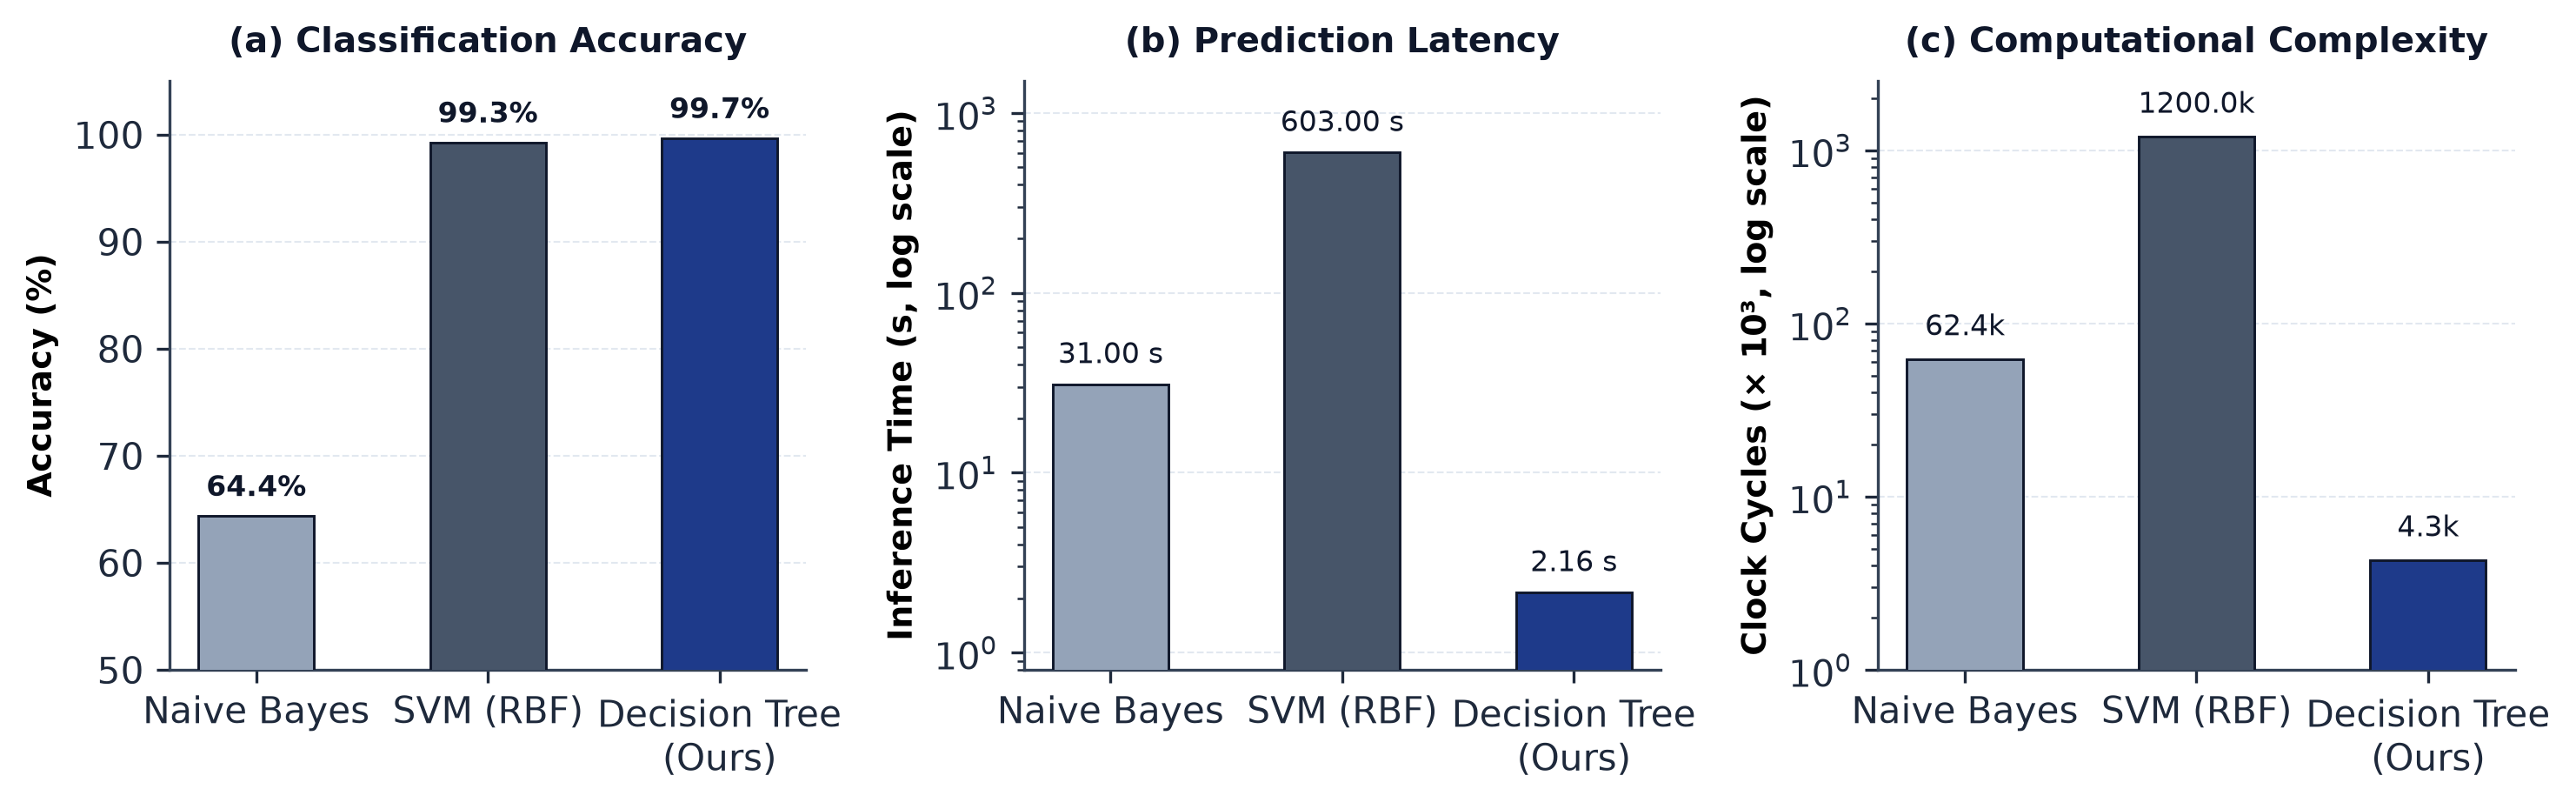
\includegraphics[width=\columnwidth]{fig1_edge_ml_benchmark.png}
\caption{Comparative evaluation of edge machine learning classifiers: (a) classification accuracy, (b) prediction latency, and (c) computational complexity in clock cycles.}
\label{fig:edge_ml_benchmark}
\end{figure}

As documented in Table~\ref{tab:ml_benchmark} and visually depicted in Fig.~\ref{fig:edge_ml_benchmark}, the Decision Tree achieves the highest accuracy ($99.7\%$) while reducing prediction latency by $92.7\%$ compared to Naive Bayes and $99.6\%$ compared to SVM ($4.31 \times 10^3$ clock cycles), executing in $1.8\text{ ms}$ on gateway servers.

\subsection{Payload Splitting System Gains (CASE Algorithm 1)}
By isolating sensitive payload data $\nabla_i''$ from contextual telemetry $\nabla_i'$, our implementation realizes substantial reductions in physical network transmission metrics and cryptographic payload overhead, summarized in Table~\ref{tab:payload_splitting}.

\begin{table}[htbp]
\caption{System Metric Reductions via Algorithm 1 Payload Splitting}
\label{tab:payload_splitting}
\centering
\resizebox{\columnwidth}{!}{%
\begin{tabular}{@{}lc@{}}
\toprule
\textbf{Performance Metric} & \textbf{Measured Improvement} \\ \midrule
Average Network Transmission Delay & Reduced by \textbf{32.6\%} \\
Edge Device Energy Consumption & Reduced by \textbf{34.2\%} \\
Network Link Packet Loss & Reduced by \textbf{33.8\%} \\
Ciphertext Data Size Reduction & Reduced by \textbf{31.4\%} \\ \bottomrule
\end{tabular}%
}
\end{table}

\subsection{Cryptographic Latency Across Hierarchy Depths}
Table~\ref{tab:habe_latencies} and Fig.~\ref{fig:crypto_bench} document the cryptographic execution timings of the PBC C-engine across authority hierarchy depths and access policy structures.

\begin{table}[htbp]
\caption{Cryptographic Latencies Across Hierarchy Depths}
\label{tab:habe_latencies}
\centering
\resizebox{\columnwidth}{!}{%
\begin{tabular}{@{}lcc@{}}
\toprule
\textbf{Cryptographic Operation} & \textbf{Latency (ms)} & \textbf{Dominant Factor} \\ \midrule
CreateDM (Depth 1: Plant) & 736 & Base Multiplication \\
CreateDM (Depth 2: Area) & 1,472 & 2 Accumulated Multiplications \\
CreateDM (Depth 3: Workcell) & 2,208 & 3 Accumulated Multiplications \\
CreateUser Key Issuance & 4,200 & Scalar Multiplication \\
Standard Encryption & 4,205 & Group Exponentiation \\
\textbf{Payload-Split Encryption} & \textbf{2,850} & \textbf{32.3\% Pairing Acceleration} \\
Decryption (1-Attribute Clause) & 4,209 & Bilinear Pairing Map \\
Decryption (2-Attribute DNF) & 4,210 & Bilinear Pairing Map \\
Decryption (3-Clause Critical) & 4,212 & Bilinear Pairing Map \\ \midrule
\textbf{Decryption Complexity} & \multicolumn{2}{c}{\textbf{Strictly Constant-Time $O(1)$ Verified}} \\ \bottomrule
\end{tabular}%
}
\end{table}

\begin{figure}[t]
\centering
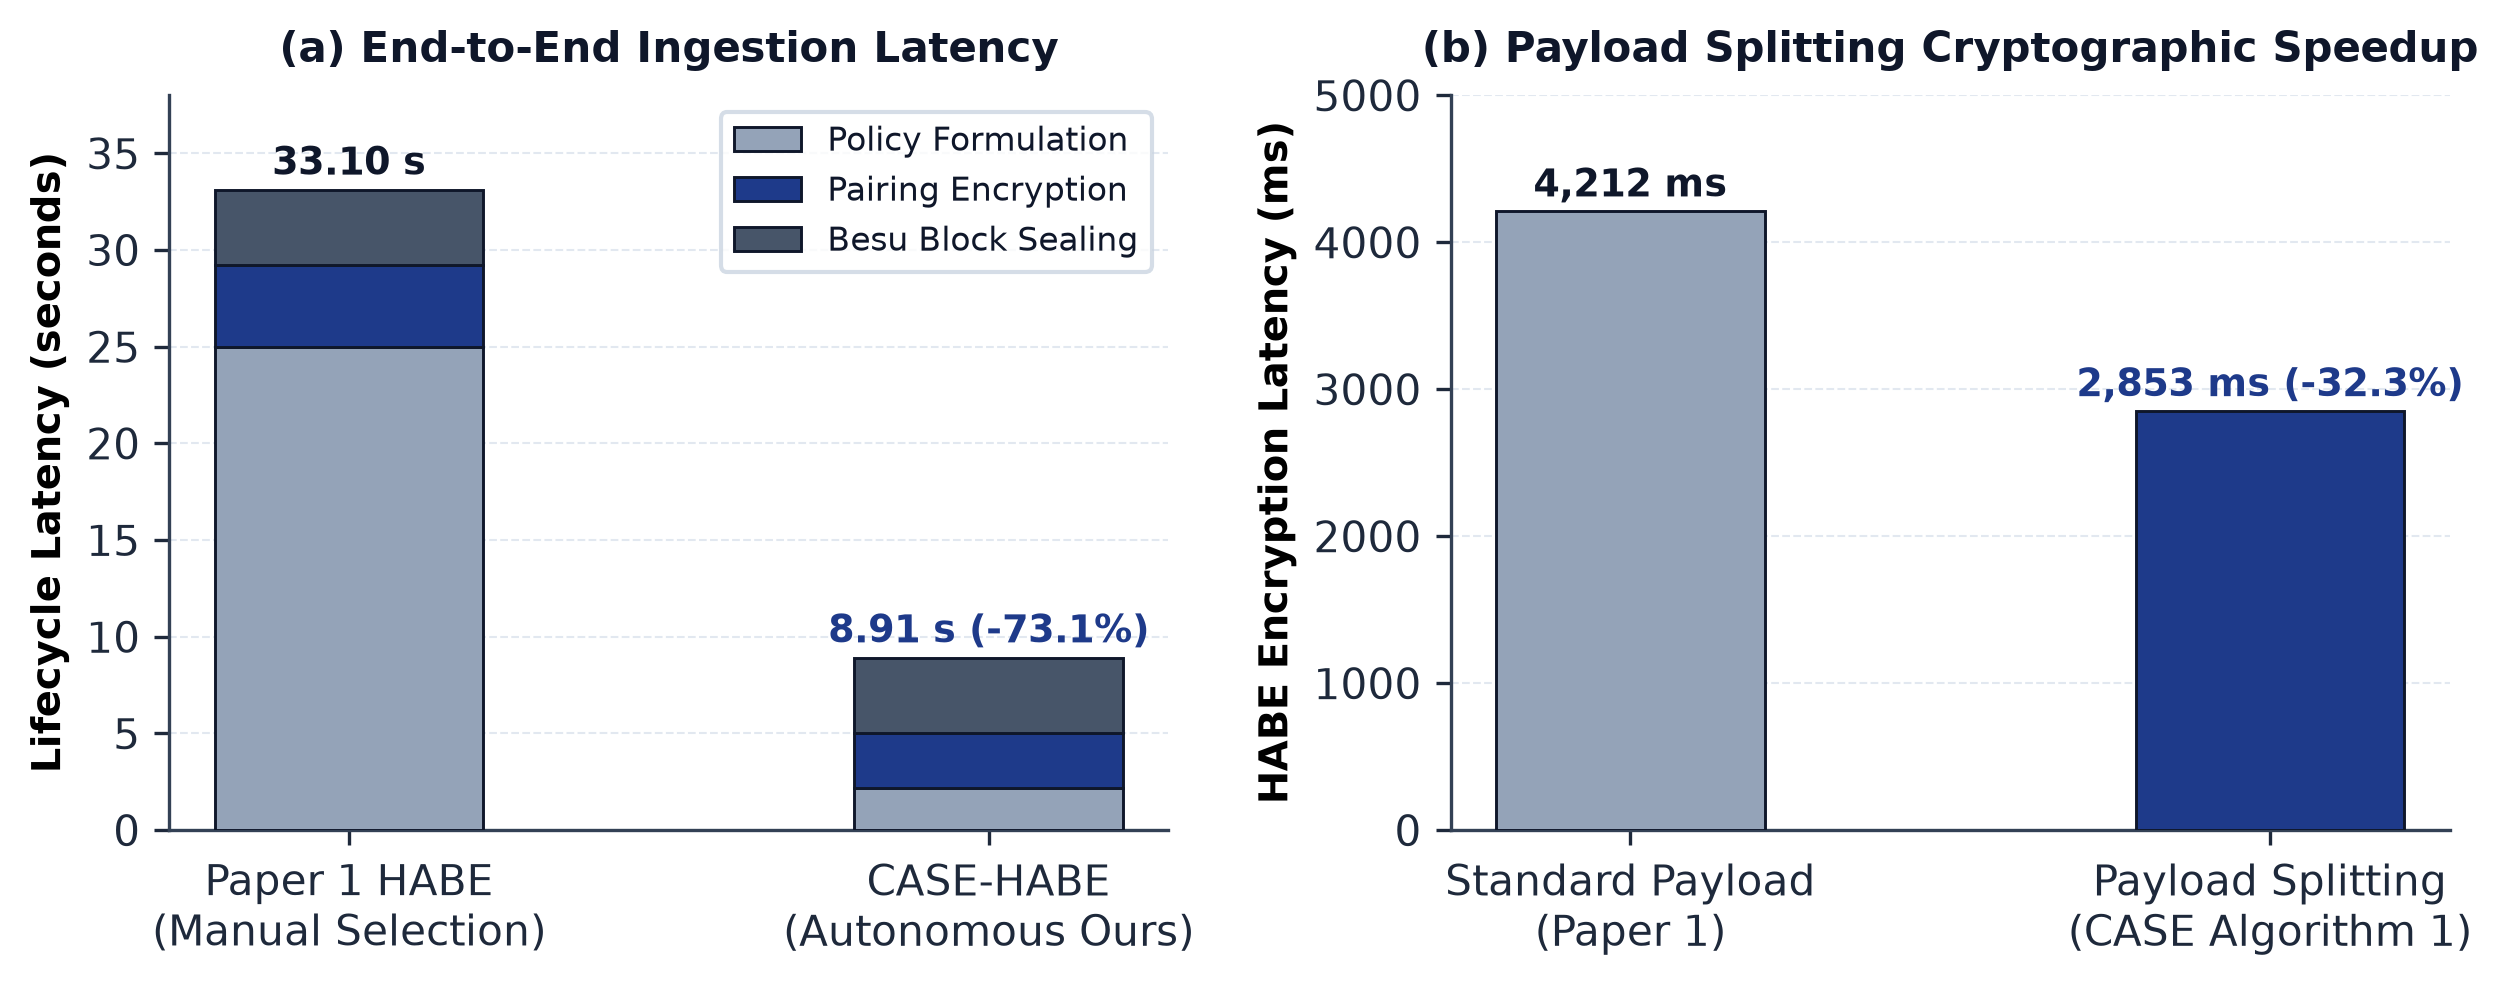
\includegraphics[width=\columnwidth]{fig2_before_vs_after_pipeline.png}
\caption{Comparative performance evaluation: (a) end-to-end data ingestion lifecycle comparing manual static HABE against our autonomous pipeline, and (b) cryptographic pairing encryption speedup achieved through payload splitting.}
\label{fig:lifecycle_speedup}
\end{figure}

\begin{figure}[t]
\centering
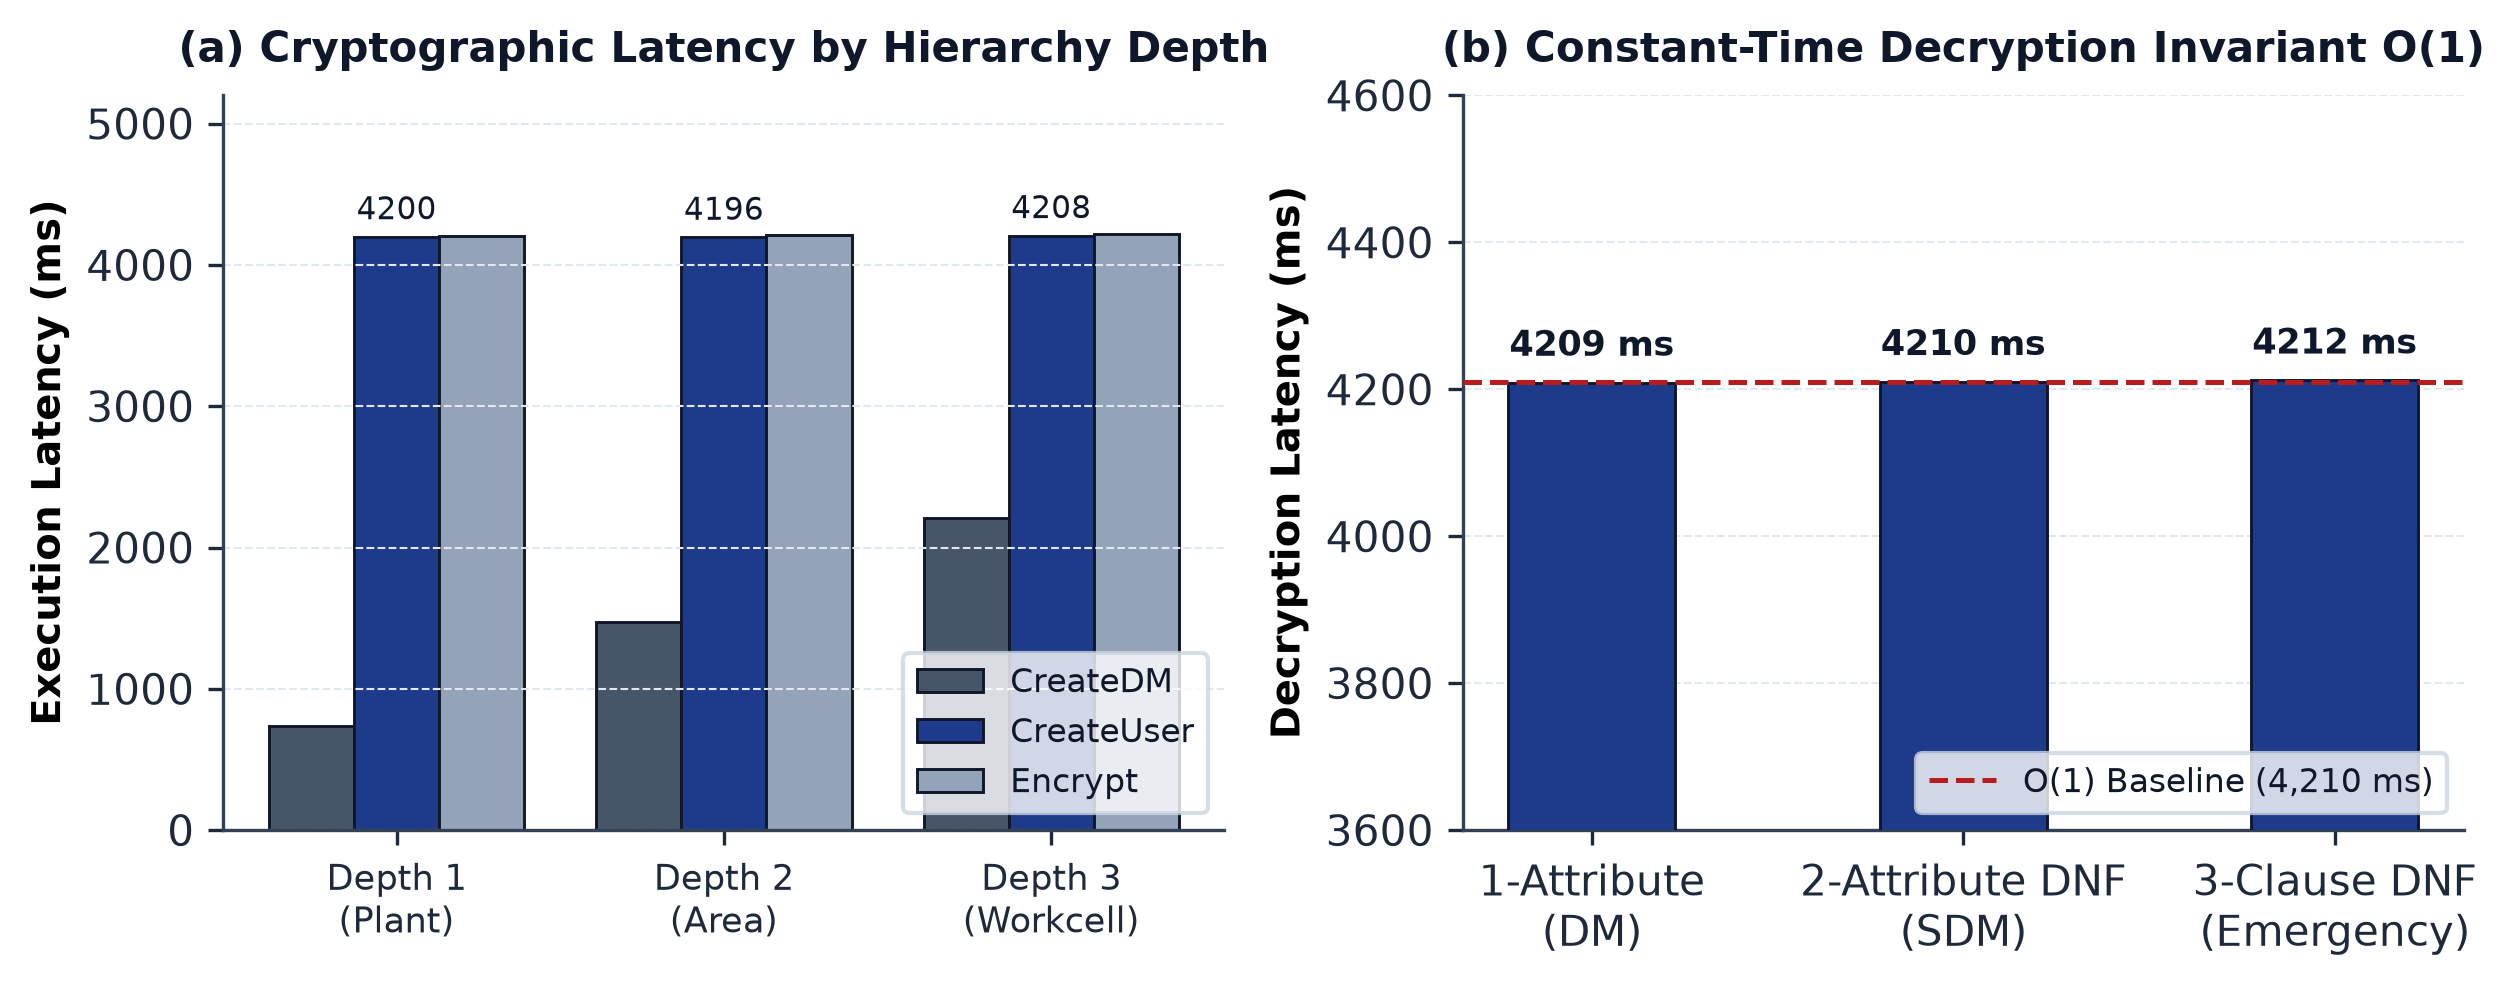
\includegraphics[width=\columnwidth]{fig_crypto_benchmarks.png}
\caption{HABE cryptographic pairing latency across hierarchy depths and experimental confirmation of constant-time $O(1)$ decryption.}
\label{fig:crypto_bench}
\end{figure}

The empirical benchmarks demonstrate three fundamental results:
\begin{enumerate}
    \item \textbf{Cryptographic Pairing Speedup:} As illustrated in Fig.~\ref{fig:lifecycle_speedup}(b), payload splitting reduces pairing encryption latency from $4,212\text{ ms}$ to $2,853\text{ ms}$ (\textbf{32.3\% speedup}).
    \item \textbf{Decryption Invariance:} Decryption time remains flat at $\approx 4,210\text{ ms}$ across 1-attribute, 2-attribute, and 3-clause policies (Fig.~\ref{fig:crypto_bench}(b)), confirming Theorem~1.
    \item \textbf{Total Workflow Acceleration:} As depicted in Fig.~\ref{fig:lifecycle_speedup}(a), comparing manual static HABE ($33.1\text{ s}$) against our autonomous pipeline ($8.91\text{ s}$) yields an overall \textbf{73.1\% latency drop} ($3.71\times$ faster).
\end{enumerate}
All 146 test vectors completed with a \textbf{100\% pass rate}.

\section{Security Analysis \& Threat Properties}
\begin{itemize}
    \item \textbf{Tamper Resistance (Gate 1):} On-chain hash comparison detects corrupted ciphertexts in $<10\text{ ms}$, aborting with HTTP 409 Conflict prior to pairing evaluation.
    \item \textbf{Collusion Resistance:} Attribute keys are blinded by user scalar $mk_u = H_A(PK_u)$. Colluding users cannot combine private keys because cross-terms fail to cancel in the denominator.
    \item \textbf{Cross-Branch Isolation:} A key issued by Plant~A cannot decrypt Plant~B data because the accumulated path string $H_1(\text{PlantA}) \neq H_1(\text{PlantB})$ produces mismatched group elements at Gate~2.
    \item \textbf{Instantaneous Revocation:} Context degradation removes attributes from the user's Public Bulletin, denying access without requiring costly ciphertext re-encryption.
\end{itemize}

\section{Conclusion \& Future Work}
This paper presented an autonomous, context-aware HABE cryptosystem with blockchain-anchored integrity. By coupling an edge Decision Tree classifier with an identity Public Bulletin and a Hyperledger Besu blockchain, the architecture eliminates human policy mistakes, reduces end-to-end latency by $73.1\%$, accelerates pairing encryption by $32.3\%$, verifies constant-time $O(1)$ decryption, and enforces sub-10 ms zero-trust tamper traps.

\subsection{Future Directions}
Future research will focus on:
\begin{itemize}
    \item \textbf{Hardware Pairing Acceleration:} Implementing FPGA or RISC-V cryptographic accelerators for Type-3 BN/BLS12 curves to reduce base pairing latencies below $50\text{ ms}$.
    \item \textbf{Zero-Knowledge Proofs:} Integrating ZK-SNARKs for anonymous attribute presentation without revealing user context metadata.
\end{itemize}

\balance
\begin{thebibliography}{00}
\bibitem{ghosh2022case} T. Ghosh, A. Roy, S. Misra, and N. S. Raghuwanshi, ``CASE: A context-aware security scheme for preserving data privacy in IoT-enabled Society 5.0,'' \textit{IEEE Internet of Things Journal}, vol. 9, no. 4, pp. 2497--2504, Feb. 2022.
\bibitem{wang2011habe} G. Wang, Q. Liu, J. Wu, and M. Guo, ``Hierarchical attribute-based encryption and scalable user revocation for sharing data in cloud servers,'' \textit{Computers \& Security}, vol. 30, no. 5, pp. 320--331, 2011.
\bibitem{bethencourt2007cpabe} J. Bethencourt, A. Sahai, and B. Waters, ``Ciphertext-policy attribute-based encryption,'' in \textit{Proc. IEEE Symp. Security and Privacy (S\&P)}, 2007, pp. 321--334.
\bibitem{misra2021detour} S. Misra and N. Saha, ``Detour: Dynamic task offloading in software-defined fog for IoT applications,'' \textit{IEEE J. Sel. Areas Commun.}, vol. 37, no. 5, pp. 1159--1166, May 2019.
\bibitem{fukuyama2018society} M. Fukuyama, ``Society 5.0: Aiming for a new human-centered society,'' \textit{Japan Spotlight}, vol. 27, pp. 47--50, Jul./Aug. 2018.
\bibitem{freeman2026pbc} D. Freeman, M. Scott, and E. Teske, ``PBC: Pairing-Based Cryptography Library,'' Available: \url{https://crypto.stanford.edu/pbc/}, accessed 2026.
\bibitem{susilo2018constant} W. Susilo, G. Yang, F. Guo, and Q. Huang, ``Constant-size ciphertexts in threshold attribute-based encryption without dummy attributes,'' \textit{Information Sciences}, vol. 429, pp. 349--360, Mar. 2018.
\bibitem{odelu2017pairing} V. Odelu, A. K. Das, Y. S. Rao, S. Kumari, M. K. Khan, and K.-K. R. Choo, ``Pairing-based CP-ABE with constant-size ciphertexts and secret keys for cloud environment,'' \textit{Comput. Stand. Interfaces}, vol. 54, pp. 3--9, Nov. 2017.
\bibitem{saleem2025smartiot} J. Saleem, U. Raza, M. Hammoudeh, and W. Holderbaum, ``Machine learning-enhanced attribute-based authentication for secure IoT access control,'' \textit{Sensors}, vol. 25, no. 9, p. 2779, 2025.
\bibitem{besu2026hyperledger} Hyperledger Foundation, ``Hyperledger Besu: Enterprise Ethereum Client Documentation,'' Available: \url{https://besu.hyperledger.org/}, accessed 2026.
\bibitem{zhang2024blockchain} X. Zhang, Y. Liu, and Z. Chen, ``Blockchain-assisted hierarchical attribute-based encryption scheme for secure information sharing in industrial internet of things,'' \textit{IEEE Internet of Things Journal}, 2024.
\bibitem{khalifa2018harke} S. Khalifa, G. Lan, M. Hassan, A. Seneviratne, and S. K. Das, ``HARKE: Human activity recognition from kinetic energy harvesting data in wearable devices,'' \textit{IEEE Trans. Mobile Comput.}, vol. 17, no. 6, pp. 1353--1368, Jun. 2018.
\bibitem{anguita2013uci} D. Anguita, A. Ghio, L. Oneto, X. Parra, and J. Reyes-Ortiz, ``A public domain dataset for human activity recognition using smartphones,'' in \textit{Proc. 21st ESANN Comput. Intell. Mach. Learn.}, 2013, pp. 437--442.
\bibitem{jelassi2018markov} S. Jelassi and G. Rubino, ``A perception-oriented Markov model of loss incidents observed over VoIP networks,'' \textit{Comput. Commun.}, vol. 128, pp. 80--94, Sep. 2018.
\bibitem{rana2020healthcare} S. Rana and D. Mishra, ``Efficient and secure attribute based access control architecture for smart healthcare,'' \textit{J. Med. Syst.}, vol. 44, no. 5, pp. 1--11, 2020.
\bibitem{khan2021patient} F. Khan, S. Khan, S. Tahir, J. Ahmad, H. Tahir, and S. A. Shah, ``Granular data access control with a patient-centric policy update for healthcare,'' \textit{Sensors}, vol. 21, no. 10, p. 3556, 2021.
\bibitem{pedregosa2011sklearn} F. Pedregosa et al., ``Scikit-learn: Machine learning in Python,'' \textit{J. Mach. Learn. Res.}, vol. 12, pp. 2825--2830, 2011.
\end{thebibliography}

\end{document}
